\documentclass[border=4pt]{standalone}
\usepackage{tikz}
\usepackage{pgfplots}
\pgfplotsset{compat=1.18}
\usetikzlibrary{shapes.geometric,arrows.meta,positioning,calc,fit,decorations.pathreplacing,backgrounds}
\definecolor{boxblue}{RGB}{225,238,252}
\definecolor{boxgreen}{RGB}{225,247,231}
\definecolor{boxorange}{RGB}{253,236,216}
\definecolor{boxgray}{RGB}{237,237,237}
\definecolor{boxred}{RGB}{253,226,226}
\begin{document}
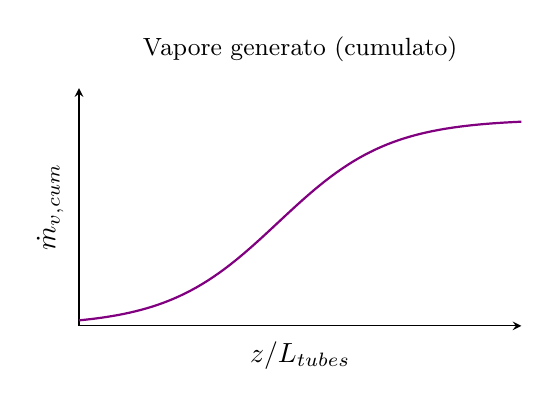
\begin{tikzpicture}
\begin{axis}[
  width=7.2cm, height=4.6cm,
  xlabel={$z/L_{tubes}$}, ylabel={$\dot m_{v,cum}$},
  xtick=\empty, ytick=\empty,
  axis lines=left,
  ymin=0, ymax=1.15, xmin=0, xmax=1,
  title={\small Vapore generato (cumulato)},
]
\addplot[thick,violet,domain=0:1,samples=80]{1/(1+exp(-8*(x-0.45)))};
\end{axis}
\end{tikzpicture}
\hspace{0.4cm}
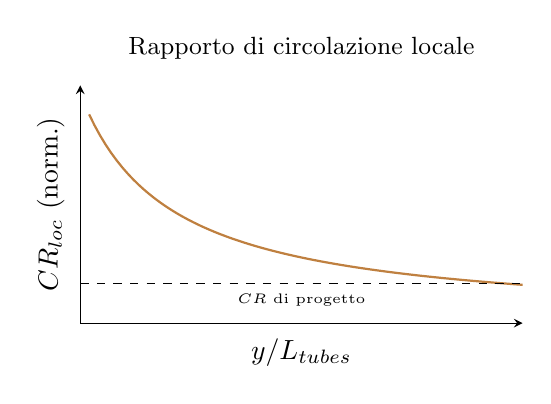
\begin{tikzpicture}
\begin{axis}[
  width=7.2cm, height=4.6cm,
  xlabel={$y/L_{tubes}$}, ylabel={$CR_{loc}$ (norm.)},
  xtick=\empty, ytick=\empty,
  axis lines=left,
  ymin=0, ymax=1.15, xmin=0, xmax=1,
  title={\small Rapporto di circolazione locale},
]
\addplot[thick,brown,domain=0.02:1,samples=80]{(1/(0.2+x))/4.5};
\draw[dashed] (axis cs:0,0.19) -- (axis cs:1,0.19) node[pos=0.5,below,font=\tiny]{$CR$ di progetto};
\end{axis}
\end{tikzpicture}
\end{document}
